\chapter{Planung}
\section{Projektziele}

\section*{Muss-Ziele}
\begin{itemize}

\item \textbf{Corporate Identity entwickeln}\newline
Wir werden uns mit der Entwicklung des Logos und auch des Designs für das WordPress Theme und für die Applikation beschäftigen.

\item \textbf{WordPress Theme entwickeln}\newline
Wir werden unser eigenes WordPress Theme und auch die verschieden Features von Grund auf neu erstellen, damit es den Wünschen des Auftraggebers entspricht. Die ganze Struktur (HTML, CSS) und auch alle Funktionen (PHP, JS) werden wir selber kodieren, und kein fertiges Layout verwenden.

\item \textbf{Theme Admin-Panel erstellen}\newline
Außer den Standardoptionen von WordPress werden wir ein zusätzliches Admin-Panel erstellen. Es soll für die Änderung von spezifischen Teilen der Seite dienen.

\item \textbf{SEO-Optimierung}\newline
Die Seite soll nach den neuesten Standards erstellt werden (HTML5, CSS3) und das ist auch Teil der SEO-Optimierung. Zusätzlich bringt dies den Effekt von höheren Rankings in Suchmaschinen wie Google, Yahoo, Bing etc.

\item \textbf{Android Applikation entwickeln}\newline
Wir werden uns mit der Entwicklung der Applikation, die entlang der Website laufen wird, beschäftigen. Sie wird dazu dienen die neuesten Artikel mit Foto- oder Video-Previews anzuzeigen, somit der Benutzer einen schnellen Blick auf den Artikel bekommt. Für eine mehr personalisierte Benutzererfahrung kann man sich auch mit sein eigenes Konto einloggen und bestimmte Topics auswählen, somit man nur die gewünschten Artikel sehen kann.

\item \textbf{Newsletter und RSS-Feed}\newline
Wenn jemand sich kein Konto erstellen will, dann steht auch die Möglichkeit sich an der wöchentlichen Newsletter zu abonnieren. Außerdem werden wir eine RSS-Feed erstellen, damit Benutzer die Posts mit einem RSS-Feed-Reader sich anschauen können. Natürlich wird es die Möglichkeit geben, von verschieden Kategorien zu wählen.

\item \textbf{Suchfunktion integrieren}\newline
Die Suchfunktion ist wichtig für unsere Benutzer, damit Sie nach etwas Spezifisches suchen können, deswegen werden wir sie in unserem Theme und auch in der Applikation integrieren.

\item \textbf{Zweisprachige Funktion}\newline
Der Inhalt soll nicht nur auf Englisch, sondern auch auf Deutsch zur Verfügung stehen, denn die Webseite richtet sich an ein breites Publikum. Dafür wird für den Administrator die Möglichkeit eingerichtet einen Artikel in beide Sprachen zu verfassen. 

\item \textbf{Sicherung von SQL-Injections}\newline
Unsere Webseite soll natürlich von SQL-Injections gesichert sein. Nachdem wir das Theme gebaut haben, werden wir nach Lücken suchen und diese Verbessern.
\end{itemize}

\section*{Optionale Ziele (Soll-, Kann-Ziele)}
\begin{itemize}
\item \textbf{Werbung durch soziale Medien}\newline
Wir werden für die Verbreitung der Webseite und Applikation sorgen, indem wir Werbung in sozialen Medien wie: Facebook, Instagram, Twitter usw. machen.
\item \textbf{Registrierung- und Anmeldefunktion}\newline
Jede Person die sich interessiert für diesen Dienst, wird die Möglichkeit haben ein Konto zu erstellen mit seine Daten (Name, E-Mail, Geschlecht, Geburtsdatum, Passwort) zu erstellen. Der Kunde kann auch zwischen der Registrierung mit E-Mail-Adresse oder Facebook auswählen. Einloggen kann sich danach entweder in der Webseite oder Applikation. Damit wir eine Brute Force Attacke vermeiden, werden wir ein Limit für die Login versuche setzen.
\end{itemize}

\section{Projektplanung}
Um die Diplomarbeit erfolgreich abschließen zu k\"onnen, ist eine gute Projektplanung erforderlich. Zu diesem Punkt geh\"oren die Besprechungen im Team und die Besprechungen mit dem Projektbetreuer, Herrn Fasching. Ganz am Beginn des Projekts wurde definiert, welche technischen Mittel zu verwenden sind. Die Arbeit wurde geteilt. Es wurde eine TO-DO Liste erstellt, die zeitlich definiert war. Basierend auf den einzelnen Schritten der TO-DO Liste, sind auch Arbeitspakete beschrieben. Da steht genau beschrieben, wer was bis wann Machen soll. Wir haben auch andere Methoden verwendet wie: Netzplan, Projektstrukturplan und Meilensteine.

\subsection{Projektstrukturplan}
In der Tabelle 2.1 ist die TO-DO Liste unserer Diplomaarbeit zu sehen

\section{Projektmanagementmethode}
\subsection{Wasserfallmodell}
In der Abbildung 2.1 wird beschrieben, wie das Wasserfallmodell in unserer Diplomaarbeit angewendet wird.Die Umsetzung dieses Modell bietet uns die Vorteile, dass die Ergebnisse in jeder Phase des Projekts getestet werden koennen.Dadurch koennen in jedem Schritt Verbesserungen uebernommen werden.

\begin{table}[h]
\begin{center}
\begin{tabular}{ |l|l|l| } 
 \hline
 \textbf{Code} & \textbf{Bezeichnung} & \textbf{bis wann?}\\ 
 \hline
 \textbf{1.} & \textbf{Recherche und Planung} &  \\ 
 \hline
 1.1 & CMS Analysieren & 23.09 \\
 \hline
 1.2 & Formulare bearbeiten & 05.09 \\
 \hline
 1.3 & Diplomarbeitsantrag abgeben & 06.09 \\
 \hline
 \textbf{2.} & \textbf{Web Dienste} & \\
 \hline
 2.1 & Domain kaufen & 05.09 \\
\hline
2.2 & Host kaufen & 05.09 \\
\hline
2.3 & CMS installieren & 24.09 \\
\hline
\textbf{3.} & \textbf{Logo} & \\
\hline
3.1 & Musterlogo erstellen & 18.09 \\
 \hline
3.2 & Finales Logo auswaehlen & 20.09 \\
\hline
3.3 & Vektor Logo erstellen & 21.09 \\
\hline
 \textbf{4.} & \textbf{Design} & \\
 \hline
 4.1 & Musterdesigns erstellen & 07.10 \\
\hline
4.2 & Finales Design auswaehlen & 10.10 \\
\hline
4.3 & Applikation Design erstellen & 12.10 \\
\hline
4.4 & Photoshop Modell zusammenstellen & 14.10 \\
\hline
 \textbf{5.} & \textbf{Wordpress Theme} & \\
 \hline
 5.1 & HTML \& CSS kodieren & 24.10 \\
\hline
5.2 & WordPress Standart CSS Classes & 28.10 \\
\hline
5.3 & Validierung des Codes & 29.10 \\
\hline
5.4 & Cross-Browser-Testung & 30.10 \\
\hline
5.5 & Testung der Aufloesung & 01.11 \\
\hline
5.6 & SEO Optimierung & 09.11 \\
\hline
5.7 & HTML \& CSS Implementierung & 30.11 \\
\hline
5.8 & CSS-Stylesheet Headers & 02.12 \\
\hline
5.9 & WordPress Page Templates & 15.01 \\
\hline
5.10 & Blog Elemente implementieren & 29.01 \\
\hline
5.11 & Registrierung und Login Bereich & 04.02 \\
\hline
5.12 & Newsletter und RSS-Feed & 07.02 \\
\hline
5.13 & SQL-Injections Testung & 12.02 \\
\hline
 \textbf{6.} & \textbf{Backend Admin Panel} &  \\ 
 \hline
 6.1 & HTML \& CSS Codierung & 15.02 \\
 \hline
 6.2 & PHP-Verbindung zu Website-Elementen & 18.02 \\
 \hline
 \textbf{7.} & \textbf{Plugins erstellen} &  \\ 
 \hline
 7.1 & Slider Plugin kodieren & 21.02 \\
 \hline
 7.2 & Instagram Feed kodieren & 24.02 \\
 \hline
  7.3 & Video Player kodieren & 27.02 \\
 \hline
\textbf{8.} & \textbf{Widgets erstellen} &  \\ 
 \hline
 8.1 & Latest Post Widget kodieren & 01.03 \\
 \hline
 \end{tabular}
 \end{center}
 \end{table}
 \newpage
 \begin{table}
 \begin{center}
 \begin{tabular}{ |l|l|l| }
 \hline
 \textbf{9.} & \textbf{Applikation} &  \\ 
 \hline
 9.1 & Android Studio installieren & 02.03 \\
 \hline
 9.2 & Projekt erstellen & 03.03 \\
 \hline
 9.3 & Tablet und Smartphone Kompatibel & 03.03 \\
 \hline
 9.4 & Kompatibilitaet mit HD und hoeher Aufloesung & 03.03 \\
 \hline
 9.5 & Java Framework auswaehlen & 03.03 \\
 \hline
 9.6 & Java Kode schreiben & 24.04 \\
 \hline
 9.6.1 & Verbindung zur Website Datenbank & 12.03 \\
 \hline
 9.6.2 & Content Layout programmieren & 20.04 \\
 \hline
 9.6.3 & Navigation Layout & 24.04 \\
 \hline
 9.7 & Applikation testen & 26.04 \\
 \hline
 9.8 & Applikation in App Store veroeffentlichen & 27.04 \\
 \hline
 \textbf{10.} & \textbf{Dokumentation} &  \\ 
 \hline
 10.1 & Status-Praesentation durchfuehren & 25.12 \\
 \hline
 10.2 & End-Praesentation durchfuehren & 24.04 \\
 \hline
 10.3 & Diplomarbeit schreiben & 30.03 \\
 \hline
 10.4 & Diplomarbeit korrigieren & 05.04 \\
 \hline
 10.5 & Diplomarbeit drucken & 14.04 \\
 \hline
 10.6 & Diplomarbeit abgeben & 24.04 \\
 \hline 
\end{tabular}
\end{center}
\caption{Arbeitsverlauf}
\end{table}

\begin{landscape}
\begin{figure}
  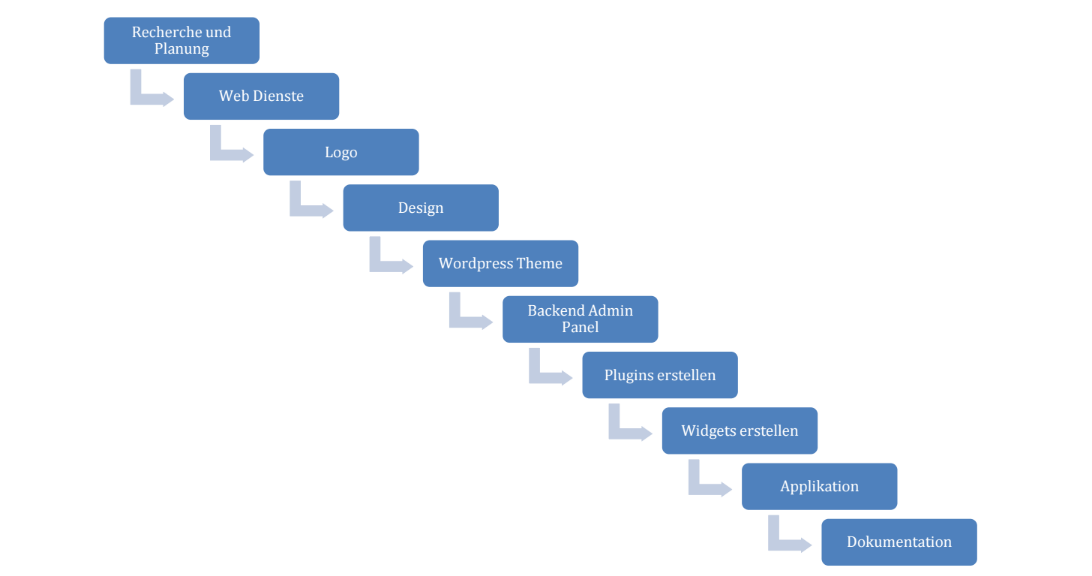
\includegraphics[width=\linewidth]{wassefall.PNG}
  \caption{Wasserfall Modell}
  \label{fig:wasserfallmodel}
\end{figure}

\end{landscape}


\chapter{Dokumentation des Projektverlaufs}


\section{Allgemeine Beschreibungen}
Das WordPress Thema ''Luxury Lust'' ist nicht nur als eine Diplomarbeit gedacht, sondern auch als eine Geschäftsidee von der Seite unserer Auftraggeber. Es ist entschieden worden, dass dieses Projekt langfristig
weiter entwickelt wird.
Das ist ein weiterer Grund, warum die Dokumentation ein sehr wichtiger
Teil dieser Diplomarbeit ist. Es muss klar und eindeutig sein, was jeder
gemacht hat. Jede Funktion, die in diese Webseite integriert wurde, ist
genau erklärt.
Die Dokumentation enthält nicht nur das Endprodukt, sondern auch die
\"Anderungen, die im Laufe der Zeit gemacht worden sind. Ziel ist es, Missverständnisse und Konflikte zu vermeiden und diese auch aufzuzeigen.
Um die Dokumentation zu schreiben, wurde entschieden, LaTeX zu
verwenden.

\section{Technische L\"osungen}
In der Tabelle 3.1 sind die technischen Lösungen zu sehen, die zur Entwicklung der Wordpress Theme dienen.

\begin{table}
\begin{center}
\begin{tabular}{ |l|l| } 
 \hline
  \textbf{F\"ur das Projekt:} & \textbf{Entscheidungen:} \\ 
 \hline
 Domain und Server & goDaddy und Bluehost \\
 \hline
 Framework & Bootstrap und Wordpress  \\
 \hline
 Formatierung und Design & HTML5, CSS3 \\
 \hline
 Funktionen & PHP, Javascript, Java \\
 \hline
 Bildbearbeitung & Adobe Photoshop, Adobe Illustrator \\
 \hline
 Daten & MySQL Datenbank, ER-Diagram \\
\hline
\end{tabular}
\end{center}
\caption{Technische Loesungen}
\end{table}

\newpage
\subsection{Bootstrap}
Für die Erstellung der Webseite ''Luxury Lust'' wurde als Framework Bootstrap verwendet. Dieses Framework ist eine Kombination aus HTML, CSS und JavaScript vorgefertigten Funktionen und Klassen. Bootstrap wird haupts\"achlich verwendet, um die Webseiten nach der Browsergr\"oße automatisch anzupassen. Diese Funktionalität war uns wichtig, damit die Seite auf Smartphones optimiert dargestellt wird.
Es gibt viele Gr\"unde, warum Bootstrap als Framework für die Webseite gew\"ahlt wurde. Der Hauptgrund ist, dass dieses Framework r\"uckw\"artskompatibel ist. So wird sichergestellt, dass die einzelnen Elemente der Website auf allen Browsern dargestellt werden k\"onnen. Ein anderer Vorteil von Bootstrap ist, dass es fertige Elemente wie Icons, Boxen, Buttons und PullDown Men\"us anbietet. Mithilfe dieser Prototypen kann man eine bessere \"Ubersicht des Designs haben. Erweiterungen wie Modal-Boxen, Tooltips und Tabs sind Teile des Frameworks, die beim Design helfen k\"onnen. Alle Elemente, die man in Boostrap findet, sind professionell gestaltet, wodurch sichergestellt wird, dass jede der m\"oglichen Komponenten einheitlich aussieht.
Dieses Framework ist anpassbar oder kann durch Erweiterungen mit neuen Funktionen versehen werden.

\subsection{goDaddy und Bluehost}
"GoDaddy ist die größte Cloud-Plattform weltweit, die sich auf kleine, unabhängige Unternehmen konzentriert. Mit mehr als 14 Millionen Kunden weltweit und mehr als 63 Millionen verwalteten Domänen ist GoDaddy der erste Ansprechpartner für Kunden mit einer Idee und dem Ziel, Kunden mit einer professionellen Website anzusprechen. Unser Ziel ist es, unseren Kunden die richtigen Tools, das Knowhow und die Unterstützung zu geben, um ihr Unternehmen erfolgreich zu machen."\footnote{Hohenberg,2016 \cite{Hohenberg2016}}

Bluehost war der Host unserer Wahl, weil es guten Kunden Support anbietet und auch eine der besten und meist verwendeten im Markt ist.

\subsection{Programmiersprachen}
Die Programmiersprachen die in diesem Projekt verwendet worden sind: 
\begin{itemize}
\item \textbf{HTML} - F\"ur den Aufbau der Website wurde die letze Version von HTML verwendet, n\"amlich HTML5.
\item \textbf{CSS} - F\"ur die Formatierung der Website wurde CSS3 verwendet, der neueste Standard von dieser Programmiersprache.
\item \textbf{JavaScript} - F\"ur den dynamischen Aufbau der Webseite wurde JavaScript mit den JQuery Libraries verwendet.
\item \textbf{PHP} - Damit wir die Website mit WordPress verbinden, verwenden wir PHP, weil das auch die Sprache von WordPress ist. Also, alle Funktionen die WordPress braucht, werden in PHP geschrieben.
\item \textbf{Java} - Die Android App werden wir in der Java Sprache schreiben, weil wir mit dieser Sprache auch in der Schule f\"ur Android Development gearbeitet haben.
\end{itemize}
\subsection{Bildbearbeitung}
\begin{itemize}
\item \textbf{Adobe Illustrator} - Wir haben dieses Programm verwendet um das Logo zu machen, weil es gut geeignet f\"ur Vektorgrafiken ist.
\item \textbf{Adobe Photoshop} - F\"ur die Mockup Entwicklung unserer Design Ideen, wurde Photoshop verwendet, weil es eines der besten Bildbearbeitungsprogramme ist.  
\end{itemize}
\begin{itemize}
\item \textbf{Daten} - F\"ur die Bearbeitung der Daten haben wir f\"ur MySQL entschieden, weil es auch die Sprache ist die von Wordpress verwendet ist. Mit eine ER Diagram werden wir darstellen die notwendigen Tabellen 
\end{itemize}






\section{Beschreibungen des Arbeitsverlaufs}
Für die Erstellung der Webseite ''Luxury Lust'' wurde als Framework Bootstrap verwendet. Dieses Framework ist eine Kombination aus HTML, CSS und JavaScript vorgefertigten Funktionen und Klassen. Bootstrap wird haupts\"achlich verwendet, um die Webseiten nach der Browsergr\"oße automatisch anzupassen. Diese Funktionalität war uns wichtig, damit die Seite auf Smartphones optimiert dargestellt wird.
Es gibt viele Gr\"unde, warum Bootstrap als Framework für die Webseite gew\"ahlt wurde. Der Hauptgrund ist, dass dieses Framework r\"uckw\"artskompatibel ist. So wird sichergestellt, dass die einzelnen Elemente der Website auf allen Browsern dargestellt werden k\"onnen. Ein anderer Vorteil von Bootstrap ist, dass es fertige Elemente wie Icons, Boxen, Buttons und PullDown Men\"us anbietet. Mithilfe dieser Prototypen kann man eine bessere \"Ubersicht des Designs haben. Erweiterungen wie Modal-Boxen, Tooltips und Tabs sind Teile des Frameworks, die beim Design helfen k\"onnen. Alle Elemente, die man in Boostrap findet, sind professionell gestaltet, wodurch sichergestellt wird, dass jede der m\"oglichen Komponenten einheitlich aussieht.
Dieses Framework ist anpassbar oder kann durch Erweiterungen mit neuen Funktionen versehen werden.
\newline
In der Tabelle 3.2 sind die Arbeitspakete und ihre Dauer in Tagen beschrieben.
\newline
\newline
\newline
\newline
\newline
\newline

\begin{table}
\begin{center}
\begin{tabular}{ |l|l|l|l| }
\hline
\textbf{Nr.} & \textbf{Arbeitsprotokoll} & \textbf{Dauer} & \textbf{Verantwortung} \\
\hline
1. & Recherche und Planung & 14 Tage & IG \\
\hline
2. & Besprechung mit Auftraggeber & 3 Tage & EP \\
\hline
3. & Beispiele im Internet finden und analysieren & 3 Tage & SK \\
\hline
4. & Name der Theme festlegen & 5 Tage & SA \\
\hline
5. & Logo erstellen & 9 Tage & IG \\
\hline 
6. & Theme skizzieren & 8 Tage & EP \\
\hline
7. & Funktionalitaet des Wordpresstheme festlegen & 7 Tage & SA \\
\hline
8. & Backup Planung & 1 Tag & EP \\
\hline
9. & Domainkaufen & 1 Tag & IG \\
\hline 
10. & PHP Framework waehlen & 2 Tage & SK \\
\hline
11. & Statische Seiten HTML & 14 Tage & SA \\
\hline
12. & Responsive Design anpassen & 6 Tage & IG \\
\hline
13. & Erste Version der Website & 2 Tage & EP \\
\hline
14. & Verbindung mit Datenbank & 1 Tag & SK \\
\hline
15. & Datenbank mit SQL erstellen & 5 Tage & SK \\
\hline
16. & Verbindung mit Datenbank testen & 2 Tage & EP \\
\hline
17. & Wordpress Page Templates & 7 Tage & IG \\
\hline
18. & Android Studio  und JDK installieren & 1 Tag & SK \\
\hline
19. & Android Studio  Tutorials analysiert & 10 Tage & SK \\
\hline
19. & Weiterarbeit an der Android Application & 15 Tage & SK \\
\hline
\end{tabular}
\end{center}
\caption{Arbeitsprotokolle}
\end{table}


Sergej Alibali[SA] ; Irza G\"er\c{c}ari[IG] ; Enso Pavaci[EP] ; Sidita Kumanova[SK]

\newpage

\section{Herausforderungen und deren Lösungen}
W\"ahrend der Umsetzung der Diplomarbeit sind ein paar Probleme aufgetreten. Zu diese Probleme sollten auch die passenden L\"osungen gefunden werden, damit das Endprodukt so gut wie m\"oglich wird.

\subsection{Fehlerhafte Layout Struktur bei Wordpress}
Auf der Abbildung 3.1 ist zu sehen wie die Posts Strukturiert sind auf unserer Webseite. Wir hatten Probleme bei der richtigen einsetzung der dazugeh\"origen CSS-Klassen.Damit wir diese gew\"unschte Struktur erreichten, haben wir mit Hilfe von unseren Projektbetreuer einen Array erstellt und auf dieses Array mit den Modulus von 4 jeweilig die gew\"unschte Klasse gesetzt.
\begin{figure}[!h]
  
\includegraphics[width=\linewidth]{post_layout.png}
  \caption{Post Layout}
  \label{fig:Post_Layout}
\end{figure} 

\newpage
\subsection*{content.php}
\begin{verbatim}
<li class="<?php set_entry_class(); ?> entry animate-box ll-article"
style="background-image: url('<?php set_featured_image_bg();
?>') ;" data-animate-effect="fadeIn">
	<div class="overlay"></div> 	
	<div class="entry-desc"> 		
	<div class="border-police">			
	<a href="<?php the_permalink(); ?>"><h3 class="mb0"><?php the_title(); 
?></h3></a>
	<p class="mb0"><?php the_time(get_option('date_format')); ?> in 
    <a href="#"><?php the_category(', '); ?></a></p>
	<p><?php print_r( excerpt(26) ); ?></p>
	</div> 	
	</div> 
</li>		

\end{verbatim}

\subsection*{functions.php}

\begin{verbatim}
function set_entry_class() {
	global $set_entry_class;
	$set_entry_class = array('two-third', 'one-third', 'one-third', 'two-third');
	global $n;
	print_r ($set_entry_class[$n%4]);
	$n++;
}
\end{verbatim}

\newpage
\subsection{Featured Image in WordPress}
Jedes Post hat auch das eigene Hintergrundbild und unsere Idee ist es das jedes Post sein eigenes ''featured Image'' hat, welch dynamisch abgerufen wird. WordPress bietet die Einschaltung das Posts solche ''featured Images'' speichern kann. 
\begin{verbatim}
function set_featured_image_bg() {
	$thumb_id = get_post_thumbnail_id();
	$thumb_url_array = wp_get_attachment_image_src($thumb_id, 'thumbnail-size', true);
	$thumb_url = $thumb_url_array[0];
	print_r ($thumb_url);
}
\end{verbatim}
\newpage
\subsection{Android Applikation Redesign}
Wir haben ein neues Design gemacht ,weil der Auftraggerber nicht sehr zufrieden mit dem ersten Modell war.
Das neue Modell ist konzeptiert nach eine leichte Navigierung Struktur und kombiniert mit unsere basic Design Ideen die mit unsere WordPress Theme passen.

\begin{figure}[!h]
  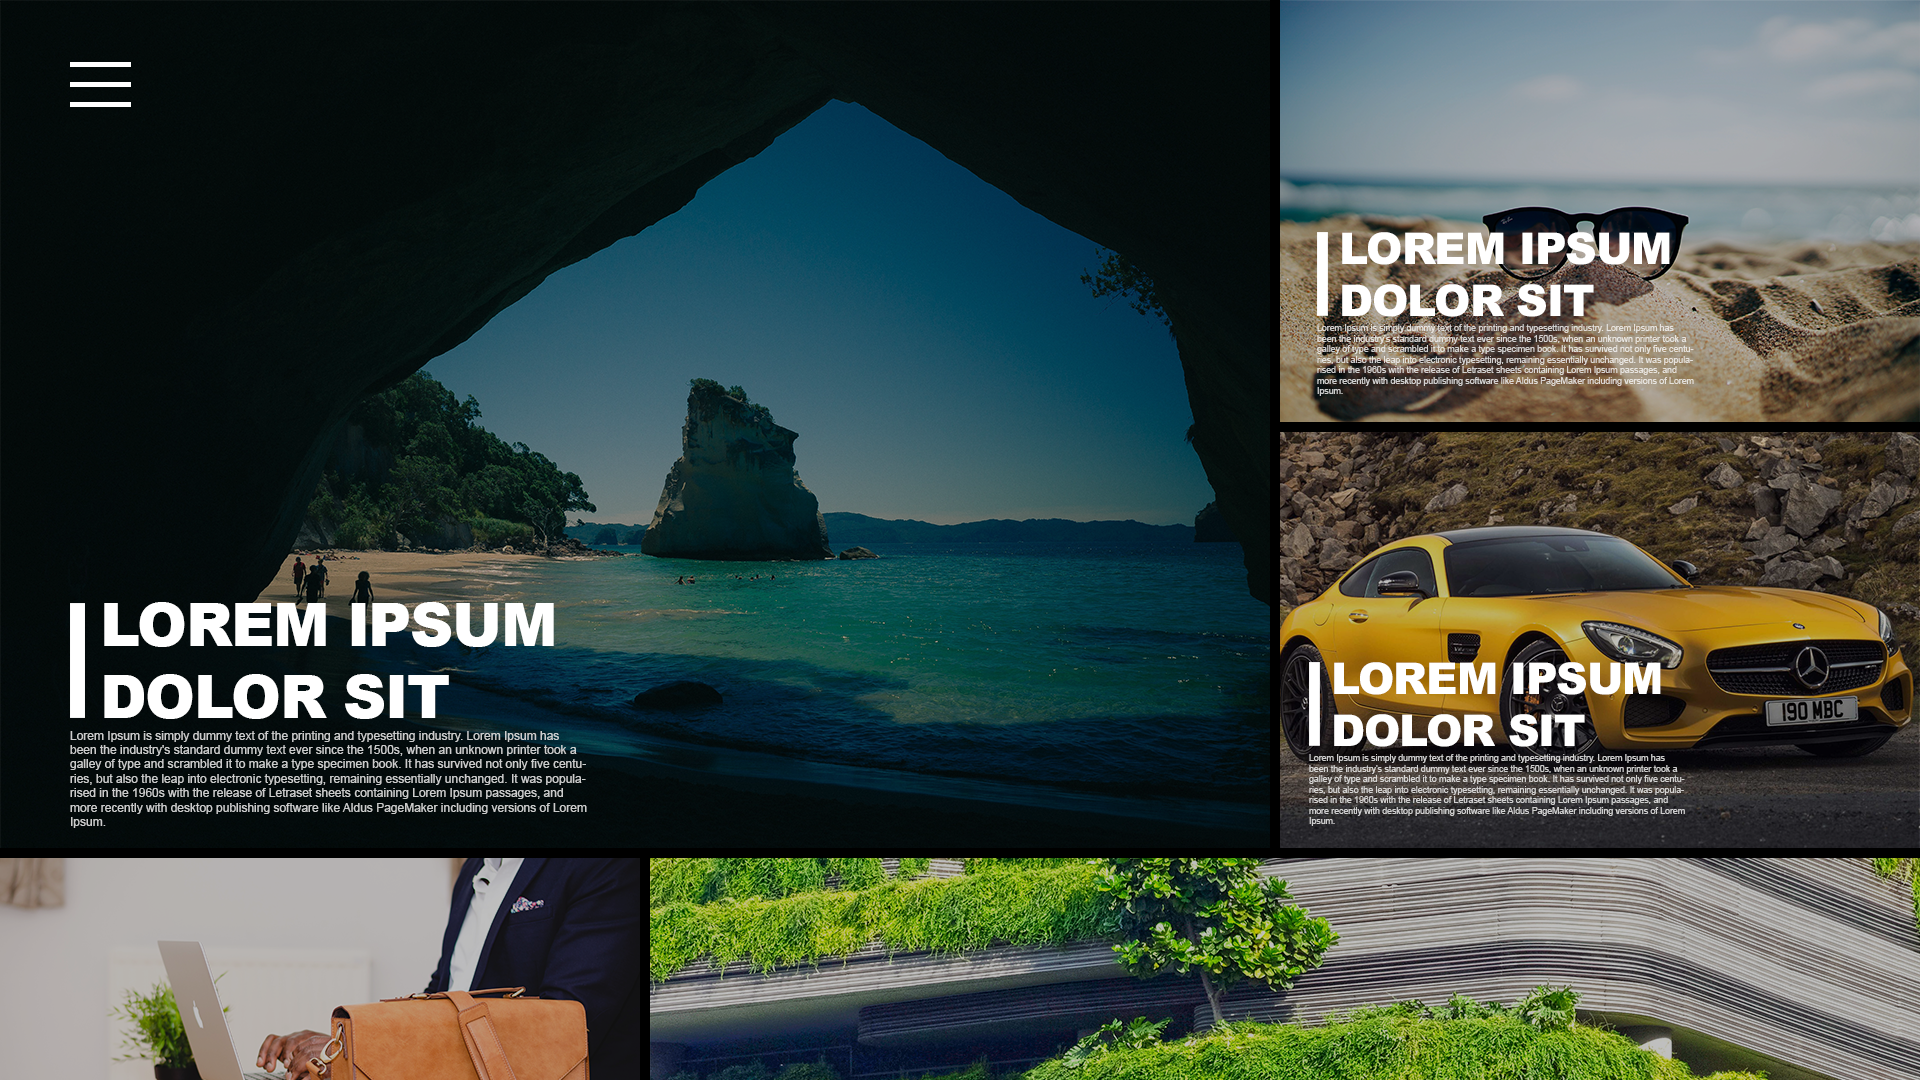
\includegraphics[width=\linewidth]{landing_tablet.png}
  \caption{Tablet}
  \label{fig:tablet}
\end{figure}

\begin{figure}[!h]
  
\includegraphics[width=\linewidth]{menu_tablet.png}
  \caption{Tablet Menu}
  \label{fig:tabletmenu}
\end{figure}

\begin{figure}[!h]
\makebox[\textwidth]{%
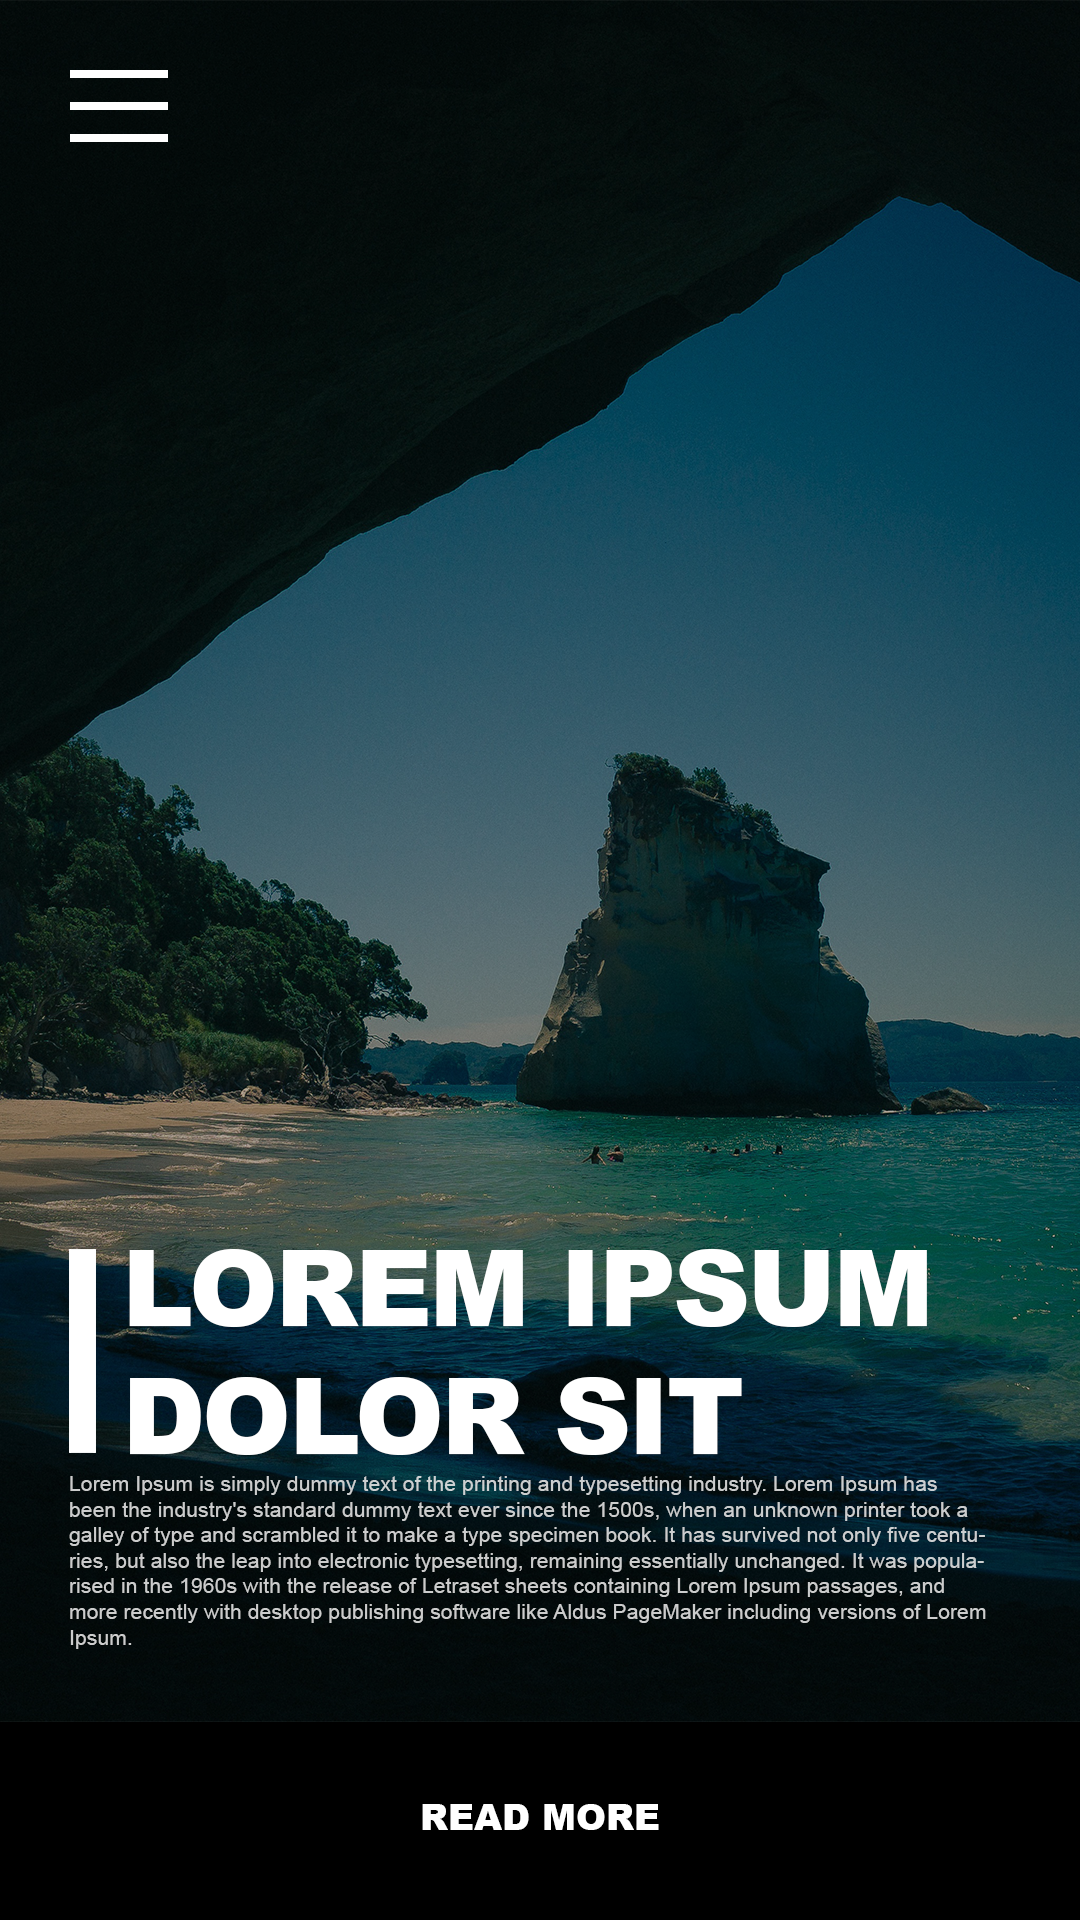
\includegraphics[width=0.30\textwidth]{landing_mobile.png}%
\hfill    

\includegraphics[width=0.30\textwidth]{menu_mobile.png}%
}\\
\end{figure}

\subsection{\"Anderung des Projekttitels}
Wir wollten das Domain luxurylifetimes.com erneuern, aber der Preis war sehr hoch gestiegen und deswegen haben wir uns gedanken gemacht f\"r einen neuen Namen, wo wir auch einen Domain finden konten. Unsere neue Wahl f\"ur den Namen war Luxury Lust und wir haben den Domain myluxurylust.com gekauft.

\subsection{Optimierung des Logos}
Weil wir den Projektnamen ge\"andert haben, war es notwendig \"Anderungen beim Design zu machen.

\subsection{Hero Section und der dazugeh\"orige Inhalt}
Wenn der Benutzer zwischen der Homepage, einer Kategorie, der Custom Templates oder einen Post navigiert, soll auch der dazugeh\"orige Hero Section (Jumbotron) angezeigt. Es ist das Problem gekommen das der Hero Section erstmals gar nicht angezeigt wurde. Nach der L\"osung dieses Problems, ist es gekommen das dasselbe gezeigt wurde auf jeder Seite. Das Problem wurde erhebt mit einer IF Anweisung, dass die Aktuelle Seite pr\"uft und den dazugeh\"origen Hero Section zeigt. 

\section{Qualitätssicherung}

\subsection{4-Augen- Prinzip}
Alle Texte, Dokumente und Erzeugnisse, die von uns erstellt werden,
werden durch einen zweiten Mitarbeiter geprüft und freigegeben, bevor
sie denitiv in die Diplomarbeit geschrieben werden. Dies gilt
gleichermaÿen für Texte, Bilder, Anwendungen und Quellcodes.

\subsection{Agenda, Protokolle}
Grundsätzlich wird zu jedem Meeting eine Agenda erstellt, die mit allen
Beteiligten im Vorfeld abgestimmt wird. Zu jedem Meeting werden die
Vereinbarungen in einem Protokoll schriftlich fixiert. Zu erwähnen ist
hier das Logbuch.

\subsection{Statuslisten}
Nach Absprache mit dem Team und unserem Betreuer erstellen wir in regelmässigem Rhythmus Statuslisten, die den jeweiligen Projektstatus mit allen Teilprojekten erfassen und neue To-Dos denieren. Diese Statuslisten werden wöchentlich aktualisiert.


\chapter{Adaptive vs. Responsive Design}


\footnote{WordPress Agentur kulturbanause® ,2015 \cite{Hellwig2015}}
\section{Adaptive Layout}
Ein Adaptive Layout ist ein für verschiedene (nicht für alle!) Displaygrößen optimiertes Web-Layout. Diese Lösung ist nicht perfekt, aber durchaus verbreitet. Der Kern des Adaptive Layouts ist ein starres Gestaltungsraster in Kombination mit Media Queries. Der gewählte Layouttyp dieser Variante ist also i.d.R. »fixed«.
Bei einem Adaptive Layout, werden verschiedene Ansichten für exakte Viewports entwickelt. Üblicherweise sind das eine Desktop-Ansicht, eine Tablet-Ansicht und eine Variante für Smartphones. Die Abmessungen der verschiedenen Ansichten orientieren sich dabei meist an bestimmten Geräten. Das iPad und das iPhone werden zu diesem Zweck gern verwendet, da die Geräte einerseits weit verbreitet sind, und darüber hinaus das mobile Internet populär gemacht haben. Im Grunde genommen wird die Website also für diese Geräte optimiert.
\begin{figure}[!h]
  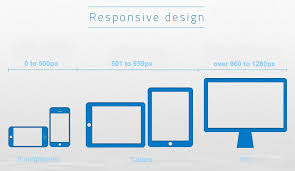
\includegraphics[width=\linewidth]{images.jpg}
  \caption{Adaptive Layout}
  \label{fig:adaptive layout}
\end{figure}
\newpage \textbf{Vorteile}
\begin{itemize}
\item Es kann gut mit klassischen Mockups, Wireframe und Skizzen gearbeitet werden, da feste Abmessungen existieren
\item Viel gestalterischer Freiraum, da mit einem starren Raster gearbeitet wird
\item Technisch recht unkompliziert umzusetzen
\item Inhalte müssen nur für klar definierte Abmessungen optimiert werden, aber nicht vollkommen flexibel sein
\item Zeitsparendere Umsetzung
\newline
\end{itemize}
\textbf{Nachteile}
\begin{itemize}
\item Häufige Fehldarstellungen auf abweichenden Endgeräten
\item Aufwändige Zielgruppenanalyse um die relevanten Viewports zu bestimmen
\item Häufig mehr CSS-Code als notwendig
\newline
\end{itemize}


\section{Responsive Layout}
Das Responsive Layout ist die bessere Lösung, um eine Seite für jede erdenkliche Displaygröße zu optimieren. Das Responsive Layout arbeitet mit einem flüssigen Gestaltungsraster, in Kombination mit Media Queries. Der Layouttyp ist demnach »fluid« oder »elastic«. Im Gegensatz zum Adaptive Layout wird hier nicht gezielt für einen bestimmten Viewport optimiert, sondern das Design so entwickelt, dass der zur Verfügung stehende Platz immer optimal ausgenutzt wird. Lediglich nach oben ist häufig eine Grenze gesetzt, damit die Website auf großen Displays nicht zu breite Spalten erhält.
Die Media Queries eines Responsive Layouts orientieren sich i.d.R. am Design und nicht an den Abmessungen eines bestimmten Displays. Die Hauptnavigation rutscht also beispielsweise dann unter das Logo, wenn das Design den Umbruch braucht, um die Information bestmöglich darstellen zu können. Das führt dazu, dass ein Responsive Layout häufig mit mehr Breakpoints bzw. Media Queries arbeitet als ein Adaptive Layout. Bei einem Responsive Layout steht das flexible Layout und die perfekte Informationsaufbereitung im Vordergrund. Bei einem Adaptive Layout steht das Ausgabegerät im Vordergrund.
\begin{figure}[!h]
  
\includegraphics[width=\linewidth]{images__1_.jpg}
  \caption{Responsive Layout}
  \label{fig:responsive layout}
\end{figure}
\newpage
\textbf{Vorteile}
\begin{itemize}
\item Jede Displaygröße wird optimal berücksichtigt
\item Es wird kein Platz verschenkt
\item Die Information steht im Vordergrund
\item Zukünftige mobile Endgeräte werden automatisch mit abgedeckt
\newline
\end{itemize}
\textbf{Nachteile}
\begin{itemize}
\item Mockups, Wireframes und Skizzen stoßen an ihre Grenzen. Häufig muss mit Prototypen gearbeitet werden um Kunden das Verhalten der Website zu zeigen
\item Komplexer in der Gestaltung
\item Komplexer in der technischen Umsetzung
\item Komplexer in der Anpassung der Seiteninhalte
\item Zeitintensivere Umsetzung
\end{itemize}


\chapter{Design}


\section{Logo}

\begin{figure}[!h]
  \centering
  \begin{minipage}[b]{0.4\textwidth}
    
\includegraphics[width=\textwidth]{bilder/logoohne.png}
    \caption{Logo 1}
  \end{minipage}
%   \hfill
%   \begin{minipage}[b]{0.4\textwidth}
%     
\includegraphics[width=\textwidth]{logomit.png}
%     \caption{Logo 2}
%   \end{minipage}
\end{figure}
In Abbildung 4.1 ist das Logo unserer Webseite zu sehen. Basierend auf unseren eigenen Ideen wir haben einige Skizzen gemacht und haben uns auf dieses entchieden. Wir haben auch ein Font dazu generiert damit unserer Logo bleibt das gleiche in verschiedenen grossen. 

Das Logo wurde mit der Software 'Adobe Photoshop' und ‚Adobe Illustrator‘ erstellt. Die ersten Buchstaben von  unserer Wordpress Theme Name nahmlich zwei ‚L‘ wurden platziert in der Mitte, gespiegelt in verschiedenen Grossen. Die Farbe des zwei Objekten ist Weiss in eine Schwarzen Hintergrund . Dann haben wir noch die ganze Name unter des Logo geschrieben. Der Kontrast ist erhoht um die ersten Blick zu bekommen. 
\section{Webseite}
\begin{figure}[!h]
  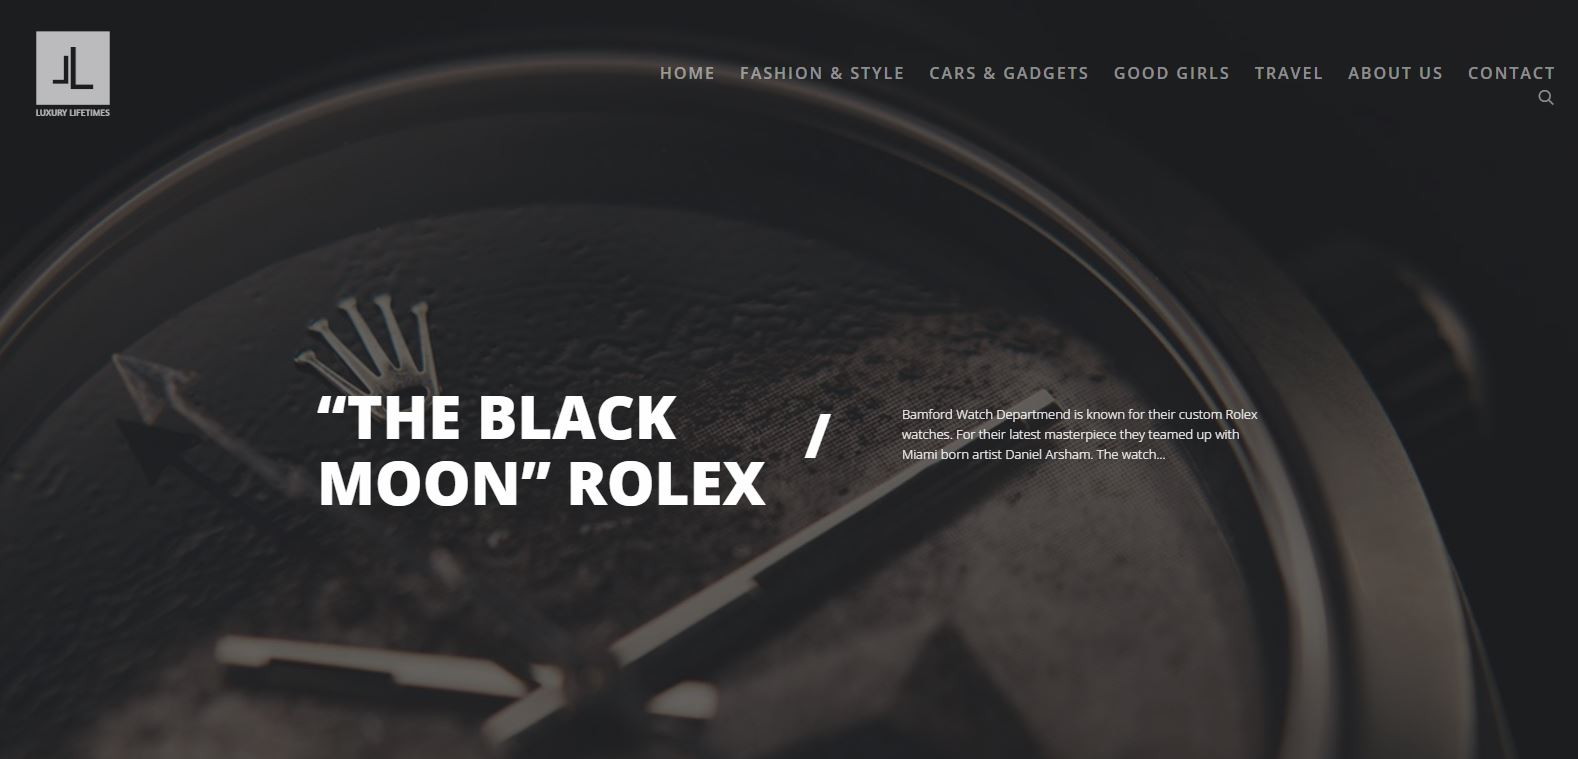
\includegraphics[width=\linewidth]{herosection1.jpg}
  \caption{Hero Section}
  \label{fig:Hero}
\end{figure}
In Abbildung 4.2.1 ist das Hero Section unserer Webseite zu sehen. Basierend auf unseren eigenen Ideen wir haben einige Skizzen gemacht und haben uns auf dieses entchieden. In unseren Hero Section ist der Navigationbar mit dem Logo auf der Linken Seite. Auf dem Hero Section wird das laetzte Post gezeigt. Ganz in der Mitte von der Post ist der Titel in Grossen und Fetten Buchstaben, ein 'Slash' als Trennlinie und eine kurze beschriftung des Posts zu sehen. Hintergrund ist die dazugehorige Photo mit einen Overlay um dunkler zu machen und die Aufmerksamkeit auf den Text zu geben.
\newpage
\begin{figure}[!h]
  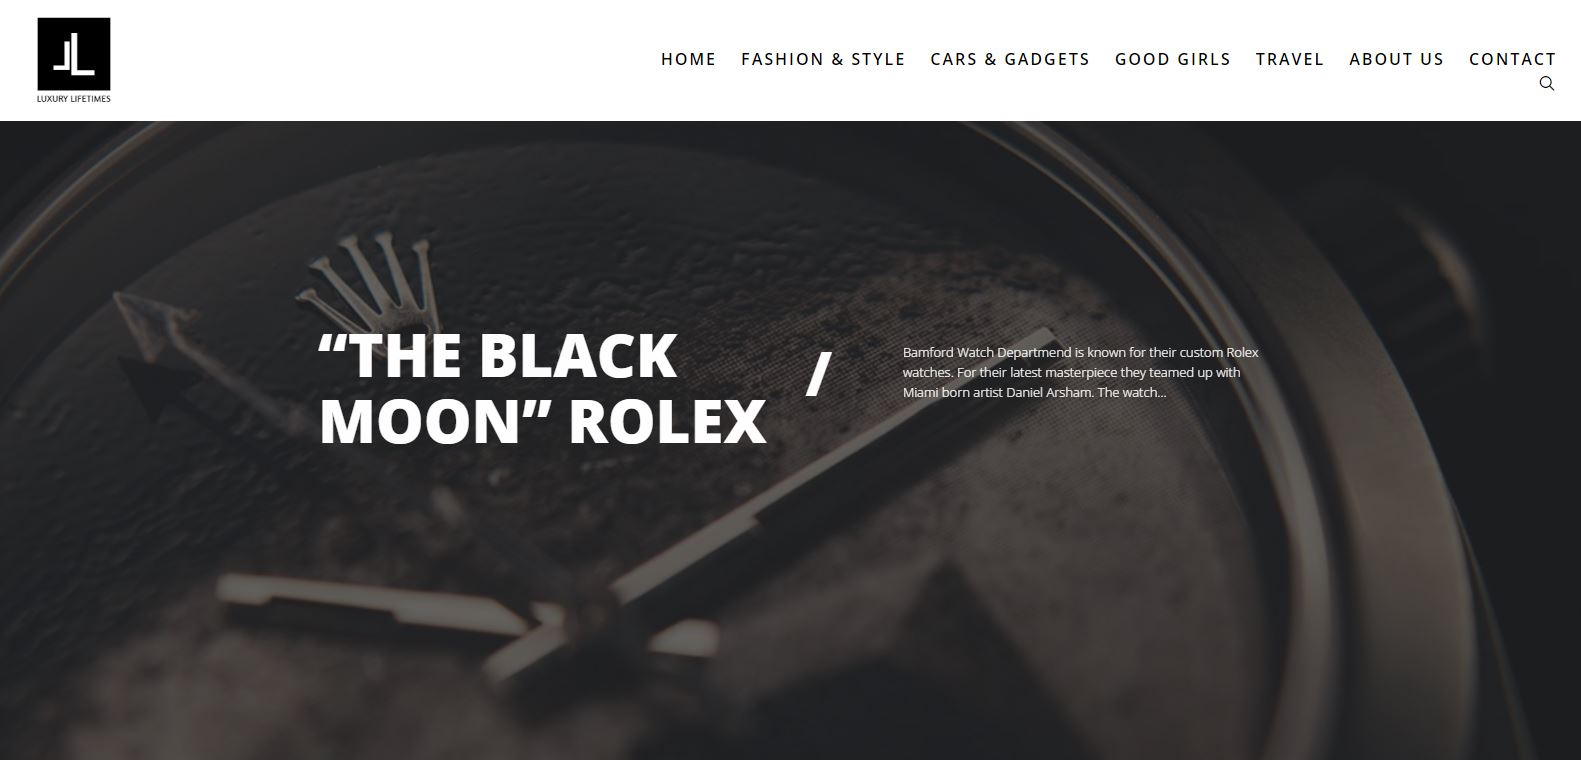
\includegraphics[width=\linewidth]{herosection1scroll.jpg}
  \caption{Hero Section Scrolled}
  \label{fig:Hero}
\end{figure}
In Abbildung 4.3.1 sieht das Hero Section so, dass die Navigations Bar von Transparent zu weiss geht, wenn wir es nach unten scrollen.
Die Farbe des Logos waechselt sich von Weiss zu Schwarz und mit der Cut-Out passiert der Gegenteil.Die Schriftfarbe der Naavigation Bar aendert sich auch von Weiss zu Schwarz. 
\newline
\begin{figure}[!h]
  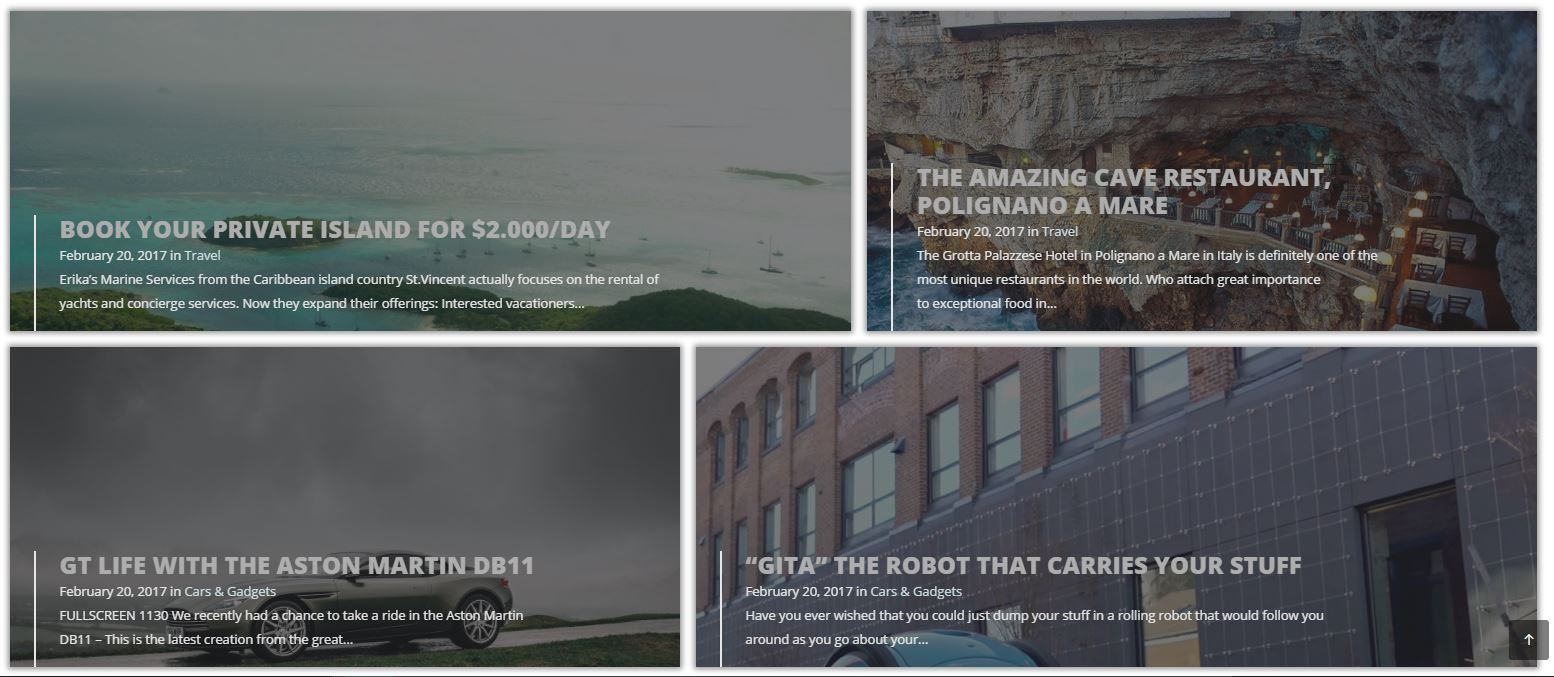
\includegraphics[width=\linewidth]{postsection1.jpg}
  \caption{Koerper }
  \label{fig:Koerper}
\end{figure}

In Abbildung 4.4.1 ist das Koper der Seite zu sehen.
Der Korper enthalt der latzten Post aber mit eine bestimmte Struktur so dass die seite auf drei Teilen geteilt ist und die Post kommen zwei drittel und ein drittel und dann umgekehrt. Zwischen den Kaestchen gibt eine feine Linie weil es besser strukturiert ausschaut.
\newline
\begin{figure}[!h]
  
\includegraphics[width=\linewidth]{footer1.jpg}
  \caption{Footer Section}
  \label{fig:footer}
\end{figure}
In Abbildung 4.5.1 ist der Footer der Seite zu sehen.
Unser Footer besteht aus ein Section mit Links fur Soziale Medien. Die haben auch ein Hover Effekt das macht die Logos 'Filled' von 'Outlined'. Ganz unten ist das Copyright Section mit den Links fur Terms Of Use und About Our Ads, sowie ein Textfeld wo unsere Kunden sich fur das Newsletter anmelden konnen.
\newpage
\begin{figure}[!h]
  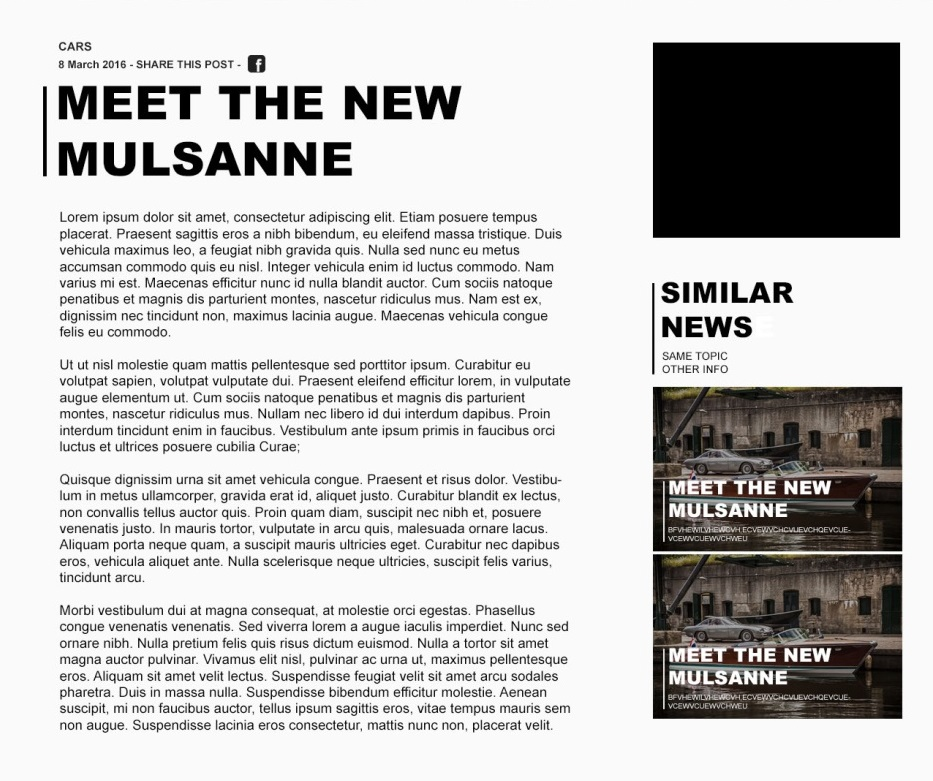
\includegraphics[width=\linewidth]{post.jpg}
  \caption{Post Section}
  \label{fig:post}
\end{figure}

In Abbildung 4.6.1 ist Post Struktur zu sehen.
Jede Post hat ein Featured Picture welche das ganze Hero Section bedeckt. Danach kommt der Post Section wo wird der Titel und ein Text sein. Oben der Titel finden wir Category woher kommt der Post , der Datum und das Author. Auf der Seite sind Relevante Posts.


\chapter{Startseite}


\section{Inhalt}
Es musste zuerst die Webseite konzipiert werden. Dazu gehört, wie die Web-seite aussehen soll und welche Funktionen sie enthalten soll. Wir sind oft im Team gesessen und haben darüber gesprochen. Es wurde festgelegt, dass die Hauptseite folgende Elemente beinhalten soll:
\begin{itemize}
\item Eine Navigationsleiste (Menu)
\item Hero Section
\item Funktionen
\item Einen Page-Footer
\end{itemize}

\section{Menu}
In diesem Punkt wurde festgelegt, dass die Inhalte des Menus wie folgt sein sollen:
\begin{itemize}
\item Home
\item Fashion \& Style
\item Cars \& Gadgets
\item Good Girls
\item Travel
\item Off-Hours
\item Search Button
\item Logo

\end{itemize}

Wenn die Browsergrösse klein ist, wird das Menu zusammengefasst, und es steht dem Benutzer ein kleiner Button zur Verfügung. So kann der Benutzer auf jedem Gerät optimal navigieren. Das wurde verwendet, um einen schöneren und klareren Überblick über die Web-seite zu haben.
\subsection*{header.php}
\begin{verbatim}
<!-- Navigationsleiste -->
<nav class="ll-nav" role="navigation">
	<div class="container-fluid">
		<div class="row">
			<!-- Logo -->
			<div class="col-xs-2 text-left">
	<div id="ll-logo"><a href="http://myluxurylust.com/wordpress/"><i class="ll-baseline-txt"></i></a></div>
				</div>
			
			<!-- Menu -->
			<div class="col-xs-10 text-right menu-1 ll-menu">
	<!-- Funktion zur Ausgabe der Menuelementen im Header Navigationsleiste -->
			<?php clean_custom_menus_header(); ?>
			</div>
		</div>
	</div>
</nav>

\end{verbatim}
\newpage
\subsection*{menu-function.php}
\begin{verbatim}
### Menu support added and registered (finished)
function register_my_menu() {
  register_nav_menu('header-menu',__( 'Header Menu' ));
  register_nav_menu('footer-menu',__( 'Footer Menu' ));
}
add_action( 'init', 'register_my_menu' );

// custom menu example @ https://digwp.com/2011/11/html-formatting-custom-menus/
function clean_custom_menus_header() {
	$menu_name = 'header-menu'; // specify custom menu slug
	if (($locations = get_nav_menu_locations()) && isset($locations[$menu_name])) {
		$menu = wp_get_nav_menu_object($locations[$menu_name]);
		$menu_items = wp_get_nav_menu_items($menu->term_id);

		$menu_list .= '<ul>' . "\n";
		foreach ((array) $menu_items as $key => $menu_item) {
		$title = $menu_item->title;
		$url = $menu_item->url;
		$menu_list .= '<li><a href="'. $url .'">'. $title .'</a></li>' . "\n";
		}
		
		//$menu_list .= '<li><i class="icon-search"></i></li>' . "\n";
		$menu_list .= '<li>' . get_search_form(false) . '</li>' . "\n";
		$menu_list .= '</ul>' . "\n";
	} else {
		// $menu_list = '<!-- no list defined -->';
	}
	echo $menu_list;
}
\end{verbatim}
\newpage


\section{Hero Section}
Ein Hero image ist ein großes Banner-Bild, das auffällig (an bevorzugtem Platz) auf der Web-Seite platziert ist, meistens am Anfang und zentriert und die ganze Bildschirmbreite einnehmend.
Das Hero image ist das erste, was ein Besucher auf unsere Website sieht, und sein Zweck ist es, einen Überblick über den wichtigsten Inhalt der Site zu geben. Es zeigt beispielsweise auf Neuigkeiten über die Site und das beziehungsweisse ist das letzte Post die addiert war.\footnote{Cousins,2016 \cite{Cousins2016}}
\begin{verbatim}
<header id="ll-header" class="ll-cover" role="banner" 
style="background-image:url('<?php set_featured_image_bg(); /*
the_post_video( $size = null ); */ ?> ');">
<div class="overlay"></div>
<div class="container">
<div class="row">
	<div class="col-xs-offset-1 col-xs-5 text-left">
	<div class="display-t">
<div class="display-tc animate-box fadeInUp animated-fast" 
data-animate-effect="fadeInUp">
<a href="<?php the_permalink(); ?>"><h1 class="mb0"><?php the_title(); ?></h1></a>
</div>
</div>
</div>
	<div class="col-xs-1 text-left">
	<div class="display-t">
	<div class="display-tc animate-box fadeInUp animated-fast" 
    data-animate-effect="fadeInUp">
	<h1 class="mb30 header-slash">/</h1>
	</div>
	</div>
	</div>
	<div class="col-xs-4 text-left">
	<div class="display-t">
	<div class="display-tc animate-box fadeInUp animated-fast" 
    data-animate-effect="fadeInUp">
	<p class="mb30 header-desc"><?php print_r( excerpt(26) ); ?></p>
	</div>
	</div>
	</div>
	</div>
	</div>
</header>
\end{verbatim}

\newpage
\section{Funktionen}
Es ist gedacht, in der Navigationsleiste zwei verschiedene Funktionen auf der Hauptseite hinzuzufügen, bzw. Suchfunktion und Sprachefunktion
\subsection{Suchfunktion}
Jede gute Webseite hat eine Suchfunktion implementiert. Auf unserer Web-seite soll es möglich sein, verschiedene Posts zu suchen.
\subsection{Sprachfunktion}
Jede gute Webseite hat eine Sprachfunktion implementiert. Auf unserer Web-seite soll es möglich sein, die Posts auf zwei Sprachen zu sehen.
\section{'About us'}
Auf der 'About Us'-Seite sollen die Kunden die Möglichkeit haben, mehrere Informationen über die Webseite 'Luxury Lust' zu erfahren.
'About us' ist eine bestimmte Seite, die im Gegenteil von die 'page.php', ruft nur das Content und nicht die ganze Posts.
\newline
\subsection*{page-aboutus.php}
\begin{verbatim}
<?php /* Template Name: About Us */ ?>

<?php get_header(); ?>
<section>
	<div id="ll-main">
		<div class="container">
			<div class="row ">
				<div class="col-md-8">
						<?php 
							if ( have_posts() ) : the_post();
										the_content();	
							endif;
						?>
				</div>
			</div>
		</div>
	</div>
</section>

<?php get_footer(); ?>



\end{verbatim}
\begin{figure}[!h]
  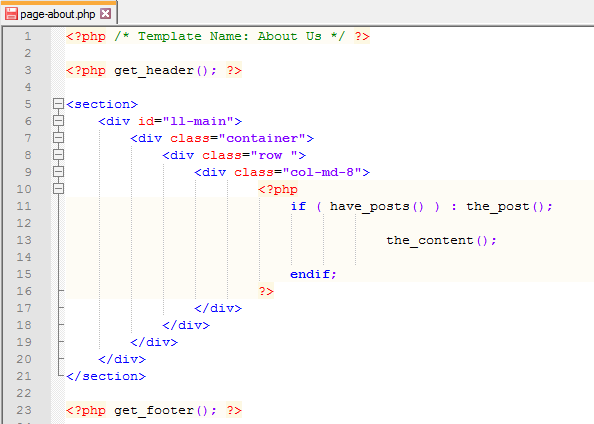
\includegraphics[width=\linewidth]{image.png}
  \caption{About Us}
  \label{fig:aboutus}
\end{figure}

\section{Posts}
Unsere Posts bestehen auf ein Bild und den Inhalt bzw. der Text. Alle Posts werden auf der Homepage und auf jede Kategorie gezeigt. Es wurde als eine List Item gestellt innerhalb eine <ul>  Tagg und es zeigt im Hintergrund ein Bilds von der Post und eine kurze Beschreibung, sowie das Datum und der Post gemacht worden ist und die Kategorie wo es gehoert. Diese Post werden automatisch geruft bis es nicht mehr gibt.


\begin{figure}[!h]
  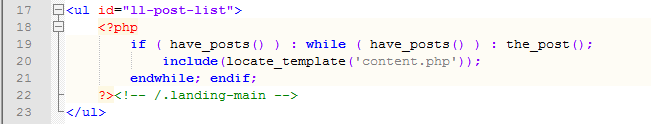
\includegraphics[width=\linewidth]{code.png}
  \caption{Post}
  \label{fig:post}
\end{figure}

\begin{figure}[!h]
  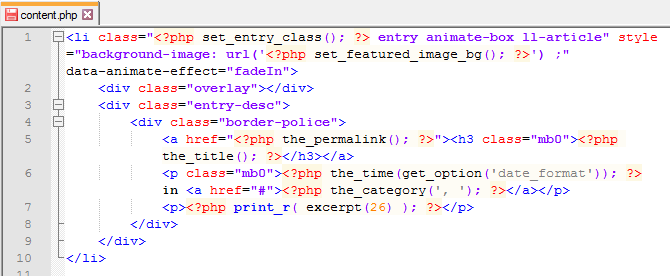
\includegraphics[width=\linewidth]{Codepost.png}
  \caption{Post}
  \label{fig:post}
\end{figure}


\chapter{Android Applikation}


\section{Java und Android}
\footnote{Trier,2016 \cite{Trier2016}}
Die entwickelte
Programmiersprache Java ist zwar mit dem Internet groß geworden, hat sich jedoch mittlerweile
als universelle, für vielfältige Zwecke einsetzbare Lösung etabliert. Unter den objektorientierten
Programmiersprachen hat Java den größten Verbreitungsgrad, und dieses Paradigma der Softwareentwicklung
hat sich praktisch in der gesamten Branche als state of the art etabliert.
Bei der Software-Entwicklung mit Java (so auch für Android) sind drei Säulen beteiligt:
\begin{itemize}
\item Die Programmiersprache - Die nach den Regeln der Programmiersprache erstellten Quellcodedateien mit den Klassendefinitionen
werden vom Compiler in Bytecode-Dateien gewandelt.
\item Die Standardklassenbibliothek mit ausgereiften Lösungen für (fast) alle Routineaufgaben
Hier bestehen Unterschiede zwischen Java-Editionen für verschiedene Einsatzfelder.
\item Die Laufzeitumgebung (virtuelle Java-Maschine) mit zahlreichen Aufgaben bei der Ausführung
von Java-Programmen
\end{itemize}

\section{JDK}
\footnote{Tutorial,2015 \cite{Tutorial2015}}
Weil es sich beim Android Studio um ein Java-Programm handelt, wird zur Ausführung auf dem
Entwicklungsrechner eine Java Virtual Maschine (JVM) benötigt. Dabei begnügt sich das Android
Studio nicht mit einer Java Runtime Environment (JRE), sondern besteht auf dem Java Software
Development Kit (JDK). Während sich die JRE auf die Rolle einer Ausführungsumgebung für JavaProgramme
beschränkt, enthält das JDK zusätzlich etliche Werkzeuge, den Quellcode der JSEStandardbibliothek
und vor allem einen Compiler, der Java-Quellcode in Byte-Code übersetzen
kann.

\section{Android Studio samt Android SDK installieren}
\footnote{Heise,2016 \cite{Heise2016}}
Android Studio ist eine kostenfreie, auf Android beschränkte Variante der kommerziell vertriebenen Entwicklungsumgebung IntelliJ IDEA. Sie bringt Funktionen mit, die Anwender sonst nur gegen Bezahlung erhalten.

Der wichtigste Unterschied zu Eclipse ist ein komplett geändertes Buildsystem namens Gradle, mit dem Entwickler jedoch nicht unbedingt in Kontakt kommen. Wegen des immensen Funktionsumfangs von Gradle beschränkt sich der Artikel auf die IDE.

\subsection{Workspace Ahoi}
\footnote{Android,2016 \cite{Android2016}}
Eclipse lagert Nutzereinstellungen und Applikationen in einem als Workspace bezeichneten Ordner. Bei IntelliJ heißt die Zusammenfassung Projekt, die Unterapplikationen nennt man Module.

Auf Android Studio umsteigende Entwickler klagen gern über die Projektflut. Das liegt daran, dass der Menüeintrag File | New Project seinem Namen gerecht wird und ein neues Projekt anlegt, was einem neuen Eclipse-Workspace entspricht. Wer ein vorhandenes Projekt um eine weitere Applikation erweitern möchte, muss stattdessen File | New Module auswählen.

\begin{figure}[!h]
  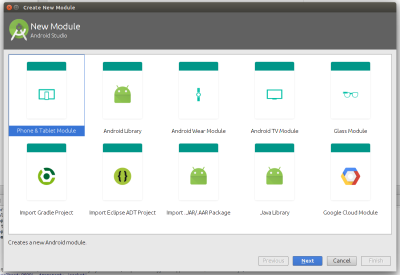
\includegraphics[width=\linewidth]{workspace.png}
  \caption{Workspace}
  \label{fig:workspace}
\end{figure}

\subsection{Nützliche Filter}
\begin{figure}[!h]
  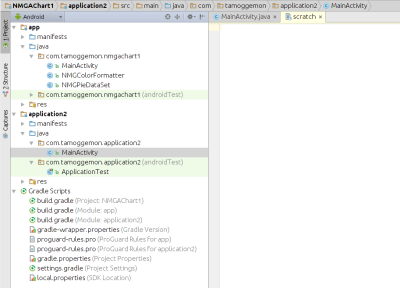
\includegraphics[width=\linewidth]{filter.png}
  \caption{filter}
  \label{fig:filter}
\end{figure}

 Projekte ufern im Laufe der Zeit aus: Eine aus mehreren tausend Codedateien bestehende Applikation ist heute keine Seltenheit mehr. Android Studio vereinfacht die Navigation an mehreren Stellen. Erstens lässt sich die in Abbildung 2 gezeigte Zeile anklicken – die linke Maustaste öffnet ein Kontextmenü, das die Inhalte der Ordnerebene anbietet.

\subsection{Fehlersuche}
Fehlersuche ist eine entscheidender Teil des Entwicklungsprozesses. Der Autor implementierte vor vielen Jahren eine Filter-Pipeline, die auf Gedeih und Verderb nur mit kleineren Datenmengen funktionieren wollte. Das Finden der Ursache nahm einige Zeit in Anspruch: Es lag im Endeffekt daran, dass das Freigeben von Ressourcen in einem Sonderfall unterblieb.

Strg + Shift + F7 hebt alle Austrittspunkte einer Methode blau hervor. Die Suche nach den Quellen bestimmter Exceptions lässt sich über dieselbe Tastenkombination bewerkstelligen, indem der Cursor über dem throws-Befehl steht.

Wer bestimmte Zeichenfolgen im Code sucht, drückt auf Strg + F. Nach der Eingabe des Suchstrings hebt der Editor relevante Passagen gelb hervor; F3 und Shift + F3 wechseln zwischen den einzelnen Resultaten.

\subsection{Vorlagen}
Applikationen zur Verwaltung mehrerer Clipboards finden in jedem Buch zur Effizienzsteigerung für Programmierer Erwähnung – klassische Zwischenablagen leiden darunter, dass sich der in ihnen befindliche Text nicht oder nur schwer an die aktuellen Gegebenheiten anpassen lässt.

Live Templates stellen eine Art permanente Zwischenablage mit diversen intelligenten Funktionen dar. IntelliJ unterteilt die Templates in folgende drei Gruppen:
\begin{itemize}
\item \textbf{Simple Live Template:} einfache Vorlage, die an der vom Cursor markierten Stelle erscheint.
\item \textbf{Parametrized Live Template:} Vorlage, die beim Einfügen mit Template-Parametern konfiguriert wird.
\item \textbf{Surround Live Template:} spezielle Variante des Simple Live Template, die den markierten Code umfasst.
\end{itemize}


\chapter{Main Activity}
\section{JSon}
\footnote{Json,2016 \cite{Json2016}}
JSON (JavaScript Object Notation) ist ein schlankes Datenaustauschformat, das für Menschen einfach zu lesen und zu schreiben und für Maschinen einfach zu parsen (Analysieren von Datenstrukturen) und zu generieren ist. Es basierd auf einer Untermenge der JavaScript Programmiersprache.
Bei JSON handelt es sich um ein Textformat, das komplett unabhängig von Programmiersprachen ist, aber vielen Konventionen folgt, die Programmieren aus der Familie der C-basierten Sprachen bekannt sind. Diese Eigenschaften machen JSON zum idealen Format für Datenaustausch.

\section{Gson}
"Gson ist eine Java-Bibliothek, die verwendet werden kann, um Java-Objekte in ihre JSON-Darstellung umzuwandeln. Es kann auch verwendet werden, um eine JSON-Zeichenfolge in ein äquivalentes Java-Objekt umzuwandeln. Gson kann mit beliebigen Java-Objekten arbeiten, einschließlich bereits vorhandener Objekte, für die Sie keinen Quellcode haben. Es gibt ein paar Open-Source-Projekte, die Java-Objekte in JSON konvertieren können. Die meisten von ihnen verlangen jedoch, dass du Java-Annotationen in deiner Klassen platzierst. Etwas, das man nicht tun kann, wenn man keinen Zugang zum Quellcode hat. Die meisten nutzen auch nicht die Verwendung von Java Generics. Gson betrachtet diese beiden als sehr wichtige Designziele."\footnote{Gson, 2017 \cite{Gson2017}}

\begin{verbatim}
Gson gson;
ProgressDialog progressDialog;
ListView postList;
Map<String,Object> mapPost;
Map<String,Object> mapTitle;
int postID;
String postTitle[];
\end{verbatim}

\section{API}
Eine Programmierschnittstelle, genauer Schnittstelle zur Anwendungsprogrammierung, häufig nur kurz API genannt, ist ein Programmteil, der von einem Softwaresystem anderen Programmen zur Anbindung an das System zur Verfügung gestellt wird.
Weil Wordpress ein API zur verfuegung stellt brauchen wir nur den Code um den Content von WP Datenbank zu rufen.

\begin{verbatim}
String url ="http://www.myluxurylust.com/wordpress/
			 wp-json/wp/v2/posts/?	
			 per_page=99&fields=id,title";
List<Object> list;
\end{verbatim}


\section{Loadscreen}
Wir haben gedacht es passt gut wenn wir ein Loadscreen hinzufuegen waehrend das App startet und die Posts geruft werden.

\begin{verbatim}
postList = (ListView)findViewById(R.id.postList);
progressDialog = new ProgressDialog(MainActivity.this);
progressDialog.setMessage("Loading...");
     progressDialog.setProgressStyle(ProgressDialog.STYLE_SPINNER);
progressDialog.show();
\end{verbatim}

\section{Objekte werden deklariert}
\begin{verbatim}
public void onResponse(String s) {
// Deklarimi i objekteve
gson = new Gson();
list = (List) gson.fromJson(s, List.class);
postTitle = new String[list.size()];
\end{verbatim}

\section{Titelspeicherung}
\begin{verbatim}
for(int i=0;i<list.size();++i){
mapPost = (Map<String,Object>)list.get(i);
mapTitle = (Map<String, Object>) mapPost.get("title");
postTitle[i] = (String) mapTitle.get("rendered");
\end{verbatim}

\section{Posts werden in List Form gezeigt}
\begin{verbatim}
// Shfaqja e cdo Postimit si liste
postList.setAdapter(new 	 ArrayAdapter(MainActivity.this,
android.R.layout.simple_list_item_1,postTitle));
progressDialog.dismiss();
\end{verbatim}

\section{Inhalt der Posts wird gerufen}
\begin{verbatim}
// Nese klikohet mbi nji Postim, ather 
do te shfaqet Postimi me permbajtjen
postList.setOnItemClickListener(
new AdapterView.OnItemClickListener() {
	@Override
public void onItemClick(AdapterView<?> parent, View view,
int position, long id) {
mapPost = (Map<String,Object>)list.get(position);
postID = ((Double)mapPost.get("id")).intValue();
\end{verbatim}

\section{Objekt deklarierung in List Form}
\begin{verbatim}
<LinearLayout xmlns:android="http://schemas.android.com/
apk/res/android"
xmlns:tools="http://schemas.android.com/tools"
android:layout_width="match_parent"
android:layout_height="match_parent"
android:paddingLeft="@dimen/activity_horizontal_margin"
android:paddingRight="@dimen/activity_horizontal_margin"
android:paddingTop="@dimen/activity_vertical_margin"
android:paddingBottom="@dimen/activity_vertical_margin"
tools:context=".MainActivity">

<!-- Deklarimi i Objektit ListView -->
<ListView
android:layout_width="match_parent"
android:layout_height="match_parent"
android:id="@+id/postList"/>
</LinearLayout>
\end{verbatim}

\chapter{Posts}
\section{Variablen deklarieren}
\begin{verbatim}
public class Post extends AppCompatActivity {
//Deklarimi i variableve
TextView title;
WebView content;
ProgressDialog progressDialog;
Gson gson;
Map<String, Object> mapPost;
Map<String, Object> mapTitle;
Map<String, Object> mapContent;
\end{verbatim}

\section{Objekspeicherung}
\begin{verbatim} 
protected void onCreate(Bundle savedInstanceState) {
super.onCreate(savedInstanceState);
setContentView(R.layout.post);

// Rujtja e Objektit te kalum prej Activity-s fillestare
final String id = getIntent().getExtras().getString("id");

title = (TextView) findViewById(R.id.title);
content = (WebView)findViewById(R.id.content);
\end{verbatim}

\section{Loadscreen}
\begin{verbatim}
// Loadscreen nderkohe qe merret Postimi
progressDialog = new ProgressDialog(Post.this);
progressDialog.setMessage("Loading...");
progressDialog.setProgressStyle(ProgressDialog.STYLE_SPINNER);
progressDialog.show();
\end{verbatim}

\section{URL die den Post ruft}
\begin{verbatim}
// URL per me marre Postimin perkates. 
ID: Kalohet nga MainActivity.java
String url = "http://www.myluxurylust.com/wordpress/wp-json/
wp/v2/posts/"+id+"?fields=title,content";
StringRequest request = new StringRequest(Request.Method.GET, url,
new Response.Listener<String>() {
    @Override
public void onResponse(String s) {
\end{verbatim}

\section{JSon Parser und Titelspeicherung}
\begin{verbatim}
// Parser per JSON edhe rujtja e Titullit + Permbajtjes
  gson = new Gson();
  mapPost = (Map<String, Object>) gson.fromJson(s, Map.class);
  mapTitle = (Map<String, Object>) mapPost.get("title");
  mapContent = (Map<String, Object>) mapPost.get("content");
\end{verbatim}

\section{Rendering im TextView und Webview}
\begin{verbatim}
// Renderi i Titullit ne TextView
title.setText(mapTitle.get("rendered").toString());

// Renderi i Permbajtjes ne WebView
content.loadData(mapContent.get("rendered").toString(),"text/html","UTF-8");
\end{verbatim}


\chapter{SoftFacts}


\section{Konfliktmanagement}
\begin{figure}[!h]
  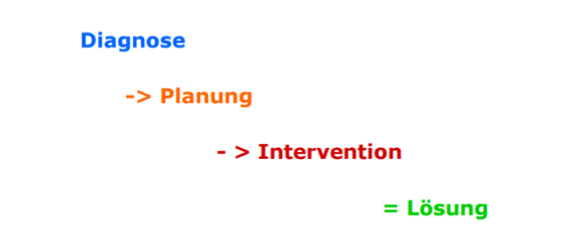
\includegraphics[width=\linewidth]{konflikte.PNG}
  \caption{Konfliktmanagement}
  \label{fig:Konfliktmanagement}
\end{figure}
Konikte sind unvermeidlich und normal. Auch in dieser Gruppe, wie auch auf alle anderen, hat es Konikte gegeben. Themen worüber Konikte gegeben hat sind:
\subsection{Design}
Jeder hat seine eigene Meinung gehabt, wenn es um das Design der Webseite gegangen wurde. Während die Besprechungen ist es sehr viel Zeit verloren, um diese Problem zu lösen.
\subsection{Termineinhaltung}
Jede Woche haben wir uns Ziele für die kommende Woche gesetzt. Es gab Fälle, wenn diese Termine nicht eingehalten wurden und das hat zu Konikte geführt. Gründe dazu waren die Mangel an Kenntnisse bzw. Beschäftigung mit andere wichtige Sachen bezüglich Schule und Matura. In diese Fälle wurden neue mehr realistische Termine vereinbart.
\subsection{Mangel an Kenntnisse}
In manche Fälle bzw. bei Der Android Applikation, war es notwendig viel Internetrecherche zu machen bzw. verschiedene Bücher zu lesen um verschiedene Aufgaben realisieren zu können. Das hat eine gewiesene Zeit gedauert.
\subsection{Krisenmanagement}
Für die Programmierung der Wordpress Theme hat es zu viel gedauert. Das war ein Problem für uns, weil bis das Theme fertig programmiert wurde, konnten die andere Teammitglieder nicht weiter arbeiten. Mit die Entwicklung dieser Hauptteil unserer Diplomarbeit, konnten die Arbeit wieder beginnen. Für eine bestimmte Zeitdauer wurde länger als im Normalfall gearbeitet.
\section{Qualitätsmanagement}
\subsection{Ursache-Wirkungsdiagramm}
In Abbildung ist die Ursache-Wirkungsdiagramm unserer Diplomarbeit zu sehen. Es wurde versucht die Hauptprobleme zu finden damit ihre Wirkungen möglichst gering bleiben.
\newpage
\begin{figure}[!h]
  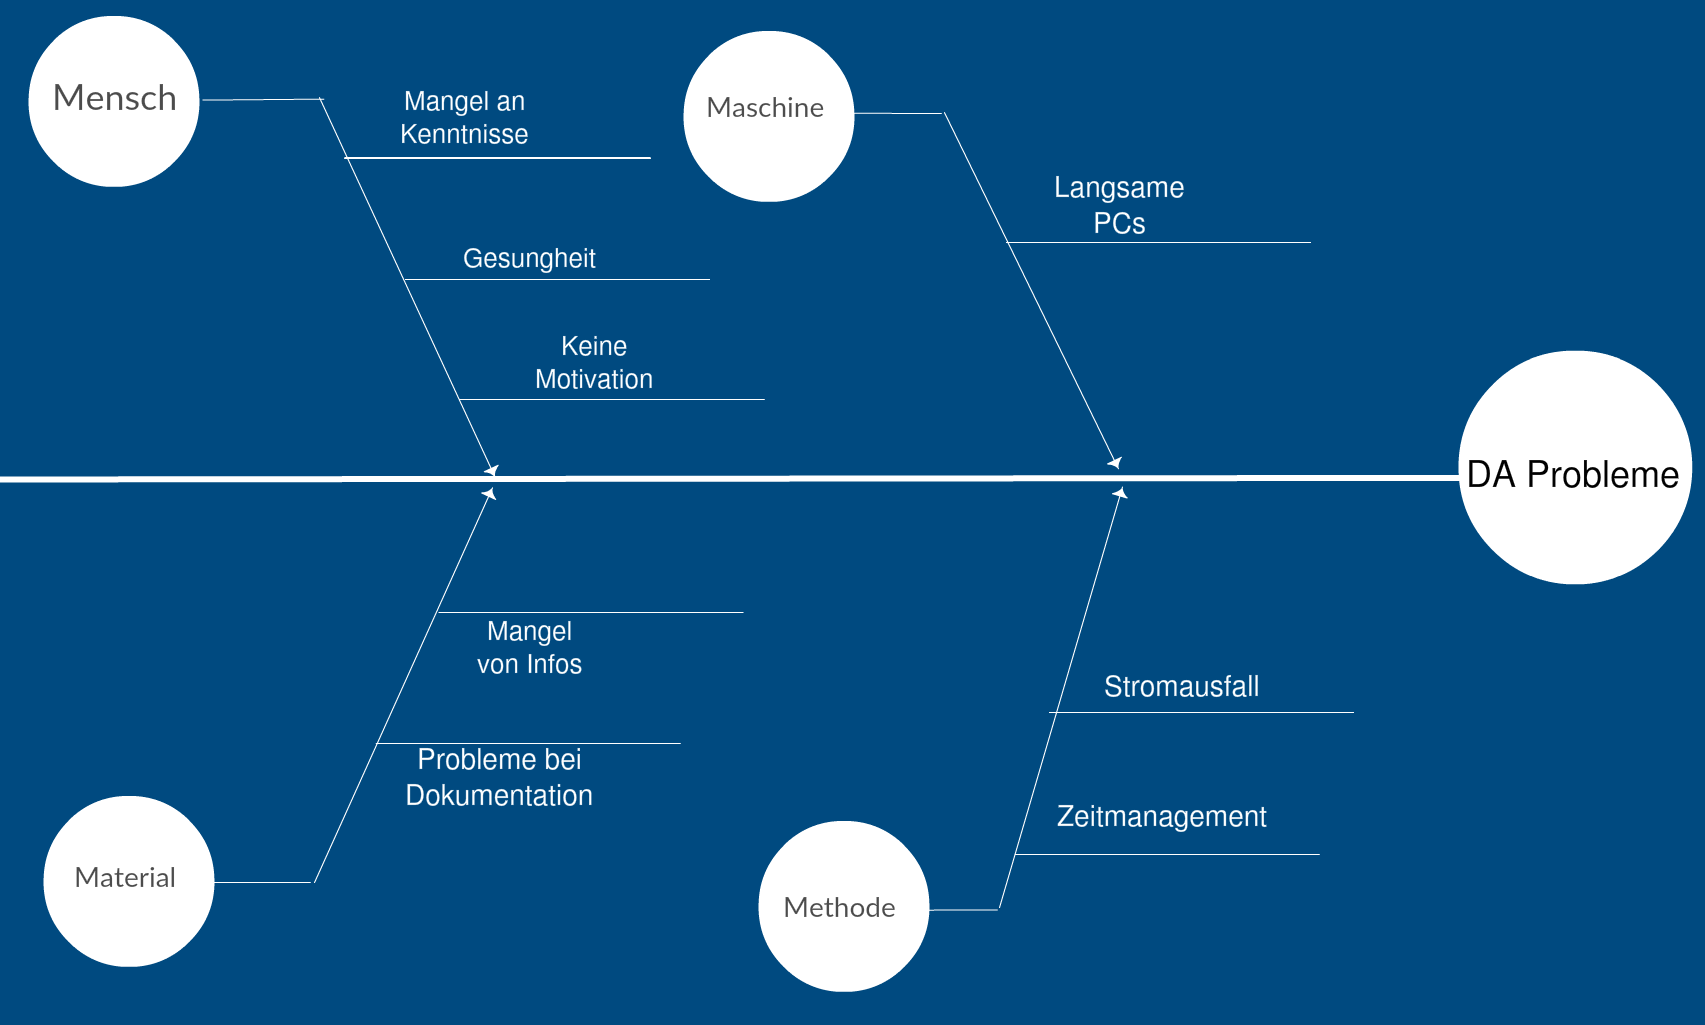
\includegraphics[width=\linewidth]{New_Fishbone_Diagram_Template_1.png}
  \caption{Diagram}
  \label{fig:Diagram}
\end{figure}

\subsection{SWOT-Analyse}
In Abbildung ist die SWOT-Analyse unserer Diplomarbeit zu sehen. Es wurden die Stärken, Schwächen, Risiken und Chancen überlegt. Es wurden Lösungen gefunden wie wir die Schwächen bzw. Chancen in Stärken und Risiken auf Chancen umwandeln können.

\subsection*{Aus Schwächen Stärken machen:}
- Falls es notwendig ist, wird es viel im Internet recherchiert und es werden verschiedene Bücher gelesen um eine passende Lösung zu finden. 
- Es wird mit unserem Projektbetreuer besprochen.

\newpage
\subsection*{Aus Chancen Stärken machen:}
-Möglichst viel Werbung machen um den Produkt berühmt zu machen.

\subsection*{Aus Risiken Chancen machen:}
- Gute Zeitmanagement. Wenn es notwendig ist, wird länger gearbeitet um die Probleme zu lösen. 
- Durch viele Internetrecherche wird es versucht die beste mögliche Programmierkonzept zu entwickeln. 
- Funktionen werden von Zeit zu Zeit analysiert, getestet und verbessert.

\begin{figure}[!h]
  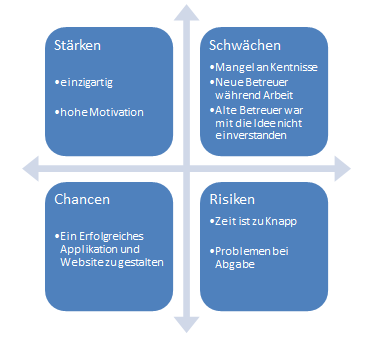
\includegraphics[width=\linewidth]{swotanalyse.PNG}
  \caption{SWOT Analyse}
  \label{fig:Swot Analyse}
\end{figure}

\chapter{Evaluierung und Resümee}
\section{Planung vs. Realisierung}
\subsection{Evaluierung der Muss-Ziele}

\begin{table}[h]
\centering
\begin{tabular}{|l|l|lll}
\cline{1-2}
\begin{tabular}[c]{@{}l@{}}\\Diese Ziel wurde erreicht\\ Es wurde ein Design fur den Website und den Android erstellt\\Das Logo wurde auch etwickelt\end{tabular}                                                                     & \textbf{Corporate Identity entwicklung} &  &  &  \\ \cline{1-2}
\begin{tabular}[c]{@{}l@{}}\\Dieses Ziel wurde erreicht\\ Es wurde selbst von uns eine eigene Theme erstellt.\\ Die ganze Struktur und alle Funktionen wurden kodiert.\end{tabular} & \textbf{Wordpress Theme entwickeln}    &  &  &  \\ \cline{1-2}
\begin{tabular}[c]{@{}l@{}}\\.....\end{tabular}                                                   & \textbf{Theme Admin-Panel erstellen}       &  &  &  \\ \cline{1-2}
\begin{tabular}[c]{@{}l@{}}\\Dieses Ziel wurde erreicht\\ Die Seite ist nach den neusten Standarts erstellt und auch Teil der SEO Optimierung\end{tabular}                                                                      & \textbf{SEO-Optimierung}       &  &  &  \\ \cline{1-2}

\end{tabular}



\caption{Evaluierung der Muss Ziele}
\end{table}

\subsection{Evaluierung der Kann-Ziele}


\chapter{Benutzerhandbuch}


\section{Hyrja tek paneli I administratorit}
Ne menyre qe te kryhen te gjitha funksionet administrative ne faqen tone,fillimisht duhet vizituar faqja :
http://myluxurylust.com/wordpress/wp-login.php

Pasi te klikoni kete link.atehere do ju hapet kjo faqe qe do ju kerkoje te dhenat tuaja.
\begin{figure}[!h]
  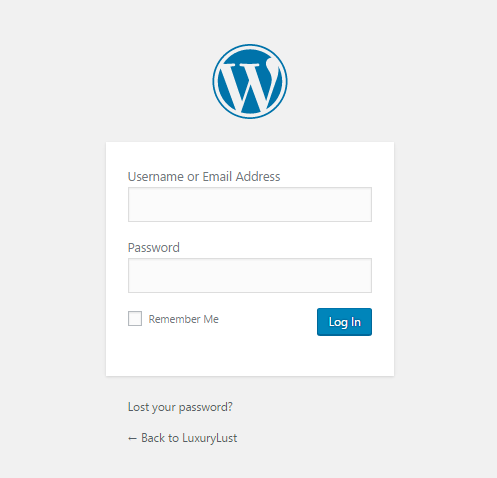
\includegraphics[width=\linewidth]{Capture.PNG}
  \caption{Log in}
  \label{fig:Log in}
\end{figure}

Ajo qe ju kerkohet eshte nje emer ose nje adrese emaili,si dhe nje password.
Ne rast se jeni I rregjistruar dhe ndodh qe te harroni passwordin,mos u shqetesoni!
Passwordin e ri mund ta merrni duke vendosur emrin apo adresen e emailit me te cilin jeni rregjistruar.

\begin{figure}[!h]
  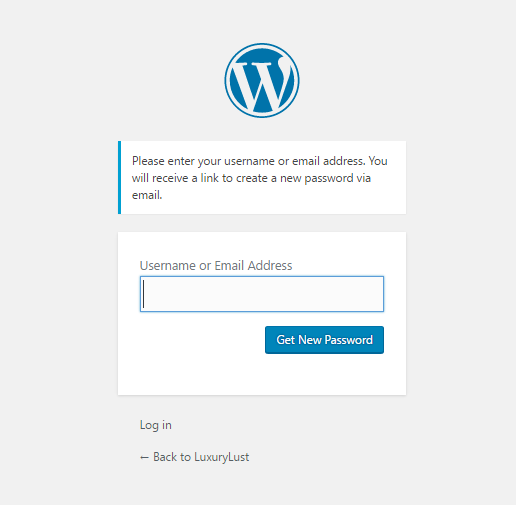
\includegraphics[width=\linewidth]{1_.PNG}
  \caption{New Password}
  \label{fig:New Password}
\end{figure}

\section{Menaxhimi I posteve}
Si ne cdo faqe tjeter updatimi I posteve eshte shume I rendesishem ne menyre qe te interesuarit e faqes te behen gjithnje e me shume ne numer,duke pasur keshtu mundesine te shtoni poste,te ndryshoni apo edhe ti fshini ato.

\begin{figure}[!h]
  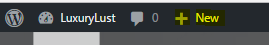
\includegraphics[width=\linewidth]{3.PNG}
  \caption{New}
  \label{fig:New}
\end{figure}
Pas klikimit te icons New do te zhvendoseni te kjo faqe qe do ju jape mundesine e postimi te nje lajmi te ri.

\begin{figure}[!h]
  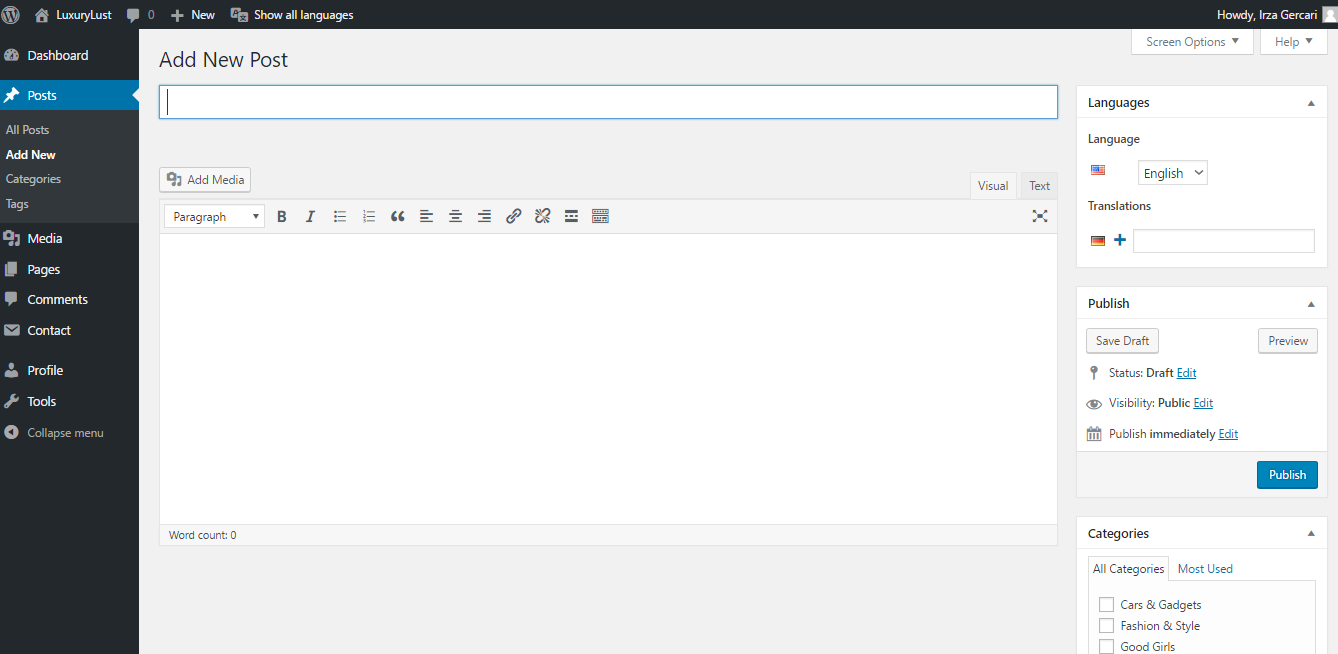
\includegraphics[width=\linewidth]{4.PNG}
  \caption{New Post}
  \label{fig:New Post}
\end{figure}

\begin{figure}[!h]
  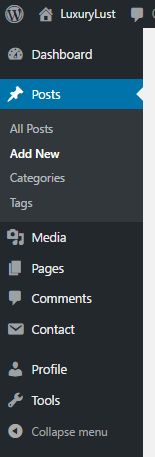
\includegraphics[width=\linewidth]{5.PNG}
  \caption{Post}
  \label{fig:New}
\end{figure}

